\documentclass[a4paper,10pt]{article}

\usepackage{amsmath}
\usepackage[utf8]{inputenc}
\usepackage{microtype}
\usepackage{hyperref}
\usepackage{tikz}

\begin{document}

\pagestyle{empty}
\noindent

\title{Udacity CarND Behavioral Cloning project}
\author{Aleksander Czechowski}
\maketitle

The purpose of this project was to train an algorithm to drive a car in a simulator,
based on recordings of human-performed driving in this simulator.
My algorithm is based on a convolutional neural network,
which matches the input from vehicle's camera with the correct steering angles.
The main goal of the project was to make the car drive one lap in autonomous mode, without leaving the road.
The objective was achieved, as documented in the video SELF\_DRIVING.mp4.

\section{Rubric points}

\subsection{Submission includes all required files and can be used to run the simulator in autonomous mode}

My project includes the following files:

\begin{itemize}
  \item clone.py, which is a Python3 script that trains the neural network;
  \item a directory train\_data, which contains data used during training
  \item model.h5, containing the trained network, that can drive the track;
  \item drive.py, which is the script that drives the car in autonomous mode;
  \item writeup/writeup.pdf, which is the project documentation you are reading now;
  \item a video file SELF\_DRIVING.mp4, serving as a proof that the car can drive one loop using the network.
\end{itemize}
 

\subsection{Submission includes functional code}

To drive the car in autonomous mode using my simulator,
run the \href{https://d17h27t6h515a5.cloudfront.net/topher/2017/February/58ae46bb_linux-sim/linux-sim.zip}{simulator} (Linux version)
and execute

\begin{center}
python drive.py model.h5
\end{center}

\subsection{Submission code is usable and readable}

The file clone.py contains the pipeline I used for creating 
The code is quite short, commented and self-documenting.

The source roughly consists of four short parts: image preprocessing, the data generator configuration, the model architecture,
and two lines of code which fit the model and save it.

\section{Model Architecture and Training Strategy}


\subsection{An appropriate model architecture has been employed}
\def\layersep{1.6cm}

Below is a \underline{schematic} drawing of the network architecture:

\begin{figure}[h]

  \begin{tikzpicture}[shorten >=1pt,->,draw=black!50, node distance=\layersep]
      \tikzstyle{every pin edge}=[<-,shorten <=1pt]
      \tikzstyle{neuron}=[circle,fill=black!25,minimum size=17pt,inner sep=0pt]
      \tikzstyle{input neuron}=[neuron];
      \tikzstyle{output neuron}=[neuron];
      \tikzstyle{hidden neuron}=[neuron];
      \tikzstyle{annot} = [text width=4em, text centered]

      % Draw the input layer nodes
      \foreach \name / \y in {1,...,6}
      % This is the same as writing \foreach \name / \y in {1/1,2/2,3/3,4/4}
          \node[input neuron] (I-\name) at (0,-\y) {};

      % Draw the conv layer nodes
      \foreach \name / \y in {1,...,6}
          \path[yshift=0.0cm]
              node[hidden neuron] (H-\name) at (\layersep,-\y cm) {};

      % Draw the max layer nodes
      \foreach \name / \y in {1,...,3}
          \path[yshift=-1.0cm]
              node[hidden neuron] (M-\name) at (3*\layersep,-\y cm) {};

      % Draw the dropout layer nodes
      \foreach \name / \y in {1,2}
          \path[yshift=-1.0cm]
              node[hidden neuron] (D-\name) at (4*\layersep,-\y cm) {};
 
      % Draw the Fully connected layer nodes
      \foreach \name / \y in {1,2}
          \path[yshift=-1.0cm]
              node[hidden neuron] (F-\name) at (5*\layersep,-\y cm) {};             

      % Draw the dropout2 connected layer nodes
      \foreach \name / \y in {1}
          \path[yshift=-1.0cm]
              node[hidden neuron] (DD-\name) at (6*\layersep,-\y cm) {};   

      % Draw the FF2 nodes
      \foreach \name / \y in {1}
          \path[yshift=-1.0cm]
              node[hidden neuron] (FF-\name) at (7*\layersep,-\y cm) {};   

      \foreach \source in {1,...,6}
              \path (I-\source) edge (H-\source);

      \foreach \source in {1,2}
         \foreach \dest in {1}
             \path (H-\source) edge (M-\dest);
      \foreach \source in {3,4}
         \foreach \dest in {2}
             \path (H-\source) edge (M-\dest);
      \foreach \source in {5,6}
         \foreach \dest in {3}
             \path (H-\source) edge (M-\dest);

      \foreach \source in {1,2}
         \foreach \dest in {1}
             \path (M-\source) edge (D-\dest);
      \foreach \source in {3}
         \foreach \dest in {2}
             \path (M-\source) edge (D-\dest);

      \foreach \source in {1,2}
        \foreach \dest in {1,2}
          \path (D-\source) edge (F-\dest);

      \foreach \source in {1,2}
        \foreach \dest in {1,2}
          \path (D-\source) edge (F-\dest);

      \foreach \source in {1,2}
        \foreach \dest in {1}
          \path (F-\source) edge (DD-\dest);

      \foreach \source in {1}
        \foreach \dest in {1}
          \path (DD-\source) edge (FF-\dest);

      % Annotate the 
 
          \node[annot,left of=I-4] {Prepro-\\ cessing: downsizing from 160x320x3 to 80x160x3, cropping to 40x160x3, normalizing from [0,255] to [-0.5,0.5]};
      \node[annot,above of=H-1, node distance=2cm] (h) {Conv. layer 16x1x1 outputs 40x160x16 tensors};
      \node[annot,left of=h] (hh) {Input layer 40x160x3 tensor};
      \node[annot,right of=h] (hl) {RELU};
      \node[annot,right of=hl] (hll) {Maxpool 2x2 outputs 20x80x16 tensor};
      \node[annot,right of=hll] (hlll) {Dropout keep\_prob =0.5};
      \node[annot,right of=hlll] (hllll) {Fully connected outputs flattened 16-dim vector};
      \node[annot,right of=hllll] (hlllll) {Dropout keep\_prob =0.7};
      \node[annot,right of=hlllll] (hllllll) {Fully connected outputs the value of steering};

  \end{tikzpicture}
 
\end{figure}

\subsection{Attempts to reduce overfitting in the model}

The model is relatively compact, so it does not overfit much in the first place.
However, two dropout layers and a maxpooling layer are in place to reduce overfitting.
In addition, during data collection the car drove the track in both directions (additional data).

\subsection{Model parameter tuning}

The model uses an adam optimizer with self-adapting learning rate.

\subsection{Appropriate training data}

The training data was collected in order for the model to learn most efficiently.
Therefore, rather than driving smoothly, which would result in a lot of 0 driving angles, 
I tried to perform many slight adjustments of the driving angles, and ``bounce'' off the edges of the road.
This allowed the network to learn recovery maneuvers.
For more details, see Subsection~\ref{CTT}.

\section{Model Architecture and Training Strategy}

\subsection{Solution Design Approach}

Initially I tried more advanced architectures (VGG, NVIDIA SDC), 
but regardless of the preprocessing, filtering (eliminating constant steering data), and regularization steps,
it would stop learning early and yield constant steering angles. Perhaps there were too many RELUs in these networks,
and they would stop learning (see \href{https://medium.com/@karpathy/yes-you-should-understand-backprop-e2f06eab496b}{Karpathy's blog, section 'dying RELU's}).
I did not find time to debug these networks at a low level. 
It is certainly worth to have a look at that problem in the future.

I performed three preprocessing steps.
First one was resizing the images, effectively reducing their resolution in half, which decreased the memory requirements for the model.
Then, I normalized the input data to have mean=0 and sigma=1, which is a standard step and allows for faster learning and easier debugging.
Both of these steps had to be repeated in the drive.py script.
Finally, I cropped 25 pixels from the top and 15 pixels from the bottom, already at the model architecture level.
The reason for cropping was that only the mid-part of the front-camera images contained relevant information on the road curvature.

\subsection{Final model architecture}

The final architecture was taken from a 'weird lame' model constructed by Cipher,
which I found while exploring \href{https://discussions.udacity.com/t/steering-stuck-hard-right/226720/24}{one of the discussions on Udacity board}.

I tried to improve Cipher's network, but it seems to be already highly optimized and performs really well at the task.
In the end, I obtained the best results by leaving it intact.

\subsection{Creation of the Training Set \& Training Process}\label{CTT}

The training data consists of 9095 images taken from the center camera.
It was not necessary to use side cameras to emulate recovery driving.
The car was being driven in both clockwise and counterclockwise directions along the track.

I tried to drive the car in a manner that would put it frequently in recovery-type situations:

\begin{figure}[h]
  \begin{center}
  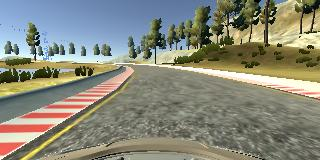
\includegraphics[width=80mm]{recovery.jpg}
\end{center}
\end{figure}

During evaluation in the simulator, the vehicle still had problems falling into water before and during the bridge. Therefore, additional data had to be collected for driving
before, and on the bridge:

\begin{figure}[h]
  \begin{center}
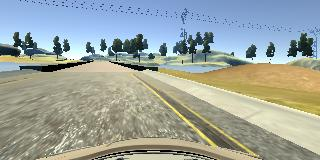
\includegraphics[width=80mm]{bridge.jpg}
\end{center}
\end{figure}

Finally, I drove an extra lap with no recovery situations, to smoothen out the driving behavior.

Some more data was collected, but it decreased the performance rather than enhancing it.
This data was excluded in driving\_log.csv, to avoid having to finetune the model again.

The model was trained for 25 epochs, with batches of 20 images, using keras ImageDataGenerator, adam optimizer and the mean squared error as the loss function
(since we are dealing with continuous range of the variable to predict).
I did not split into training/validation/test sets, as I wanted to use all the data I collected.
This was important for troubleshooting problems on specific parts of the track, I did not want the data I collected for that purpose to go into the validation part.
Instead of validation accuracy, the evaluation of the model was performed in the simulator, by successfully completing a lap without driving off the road.

The training was performed on AWS g2.2xlarge server, so the training time was reduced by the use of a GPU.

\end{document}
